\begin{frame}[t]
  \frametitle{The many-electron problem}
  Many-electron Schr{\"o}dinger equation
  \[\left\{\sum_{i=1}^N \left[ -\frac{1}{2} \nabla_i^2 - \frac{Z}{r_i} \right] + \sum_{i<j}^N \frac{1}{|\vec{r}_i - \vec{r}_j|}\right\} \Psi = E \Psi\] \pause
  \begin{itemize}
      \item {Analytical solution: \alert{$\textrm{\ding{55}}$}}
      \item {Numerical solution: \alert{$\textrm{\ding{55}}$}}
      \item {We use \emph{self-consistent field (SCF)} approximation}
  \end{itemize}
\end{frame}

\begin{frame}[t]
  \frametitle{The many-electron problem}
  \emph{Hartree} ansatz
  \[ \Psi(\vec{r}_1,\vec{r}_2,\ldots,\vec{r}_N) \approx \varphi_1(\vec{r}_1)\varphi_2(\vec{r}_2)\ldots\varphi_N(\vec{r}_N) \]
  \emph{Mean-field} approximation
  \begin{align*}
  H & = \sum_{i=1}^N \left[ -\frac{1}{2} \nabla_i^2 - \frac{Z}{r_i} \right] + \underbrace{\sum_{i<j}^N \frac{1}{|\vec{r}_i - \vec{r}_j|}}_{\text{\alert{Trouble maker}}} \\
  H & = \sum_{i=1}^N \left[ -\frac{1}{2} \nabla_i^2 - \frac{Z}{r_i} \right] + \underbrace{V_\text{Hartree}(r)}_{\text{\emph{Hartree potential}}}
  \end{align*}
\end{frame}

\begin{frame}[t]
  \frametitle{Self-consistent iteration}
  \footnotesize
  \emph{Many-electron} problem $\rightarrow$ Many \emph{one-electron} problems
  \[ \boxed{-\frac{1}{2} \frac{d^2u_i}{dr^2} + \left[ V_{\text{ext}}(r) +  \emph{V_{\text{Hartree}}(r)} + \frac{l(l+1)}{2r^2} \right] u_i = E_i u_i} \] \pause
  Chicken or the egg problem!
  \scriptsize
  \tikzstyle{cloud}    = [ellipse, draw, text width=4.0em, text badly centered, minimum height=2em]
  \tikzstyle{block}    = [rectangle, draw, rounded corners, text width=4.5em, text badly centered, minimum height=4em]
  \tikzstyle{decision} = [diamond, draw, text width=4.5em, text badly centered, aspect=1.5]
  \tikzstyle{line}     = [draw, -triangle 45]
  \Put(-130,-170){
  \begin{tikzpicture}[node distance = 9em, auto]
  % Place nodes
  \node [cloud] (init) {initial potential};
  \node [block, right of=init] (orbital) {compute \emph{$\{u_i(r)\}$}};
  \node [block, right of=orbital] (potential) {compute \emph{$V_{\text{Hartree}}(r)$}};
  \node [block, below of=potential, node distance=5em] (update) {update \emph{$V_{\text{Hartree}}(r)$}};
  \node [decision, right of=potential] (converge) {converged?};
  \node [cloud, right of=converge, text width=2.5em,] (stop) {stop};
  % Draw edges
  \path [line] (init) -- (orbital);
  \path [line] (orbital) -- (potential);
  \path [line] (potential) -- (converge);
  \path [line] (converge) |- node [near start] {no} (update);
  \path [line] (update) -| (orbital);
  \path [line] (converge) -- node {yes}(stop);
  \end{tikzpicture}
  }
\end{frame}

\begin{frame}[t]
  \frametitle{JavaScript demonstration}
  \footnotesize
  \centering
  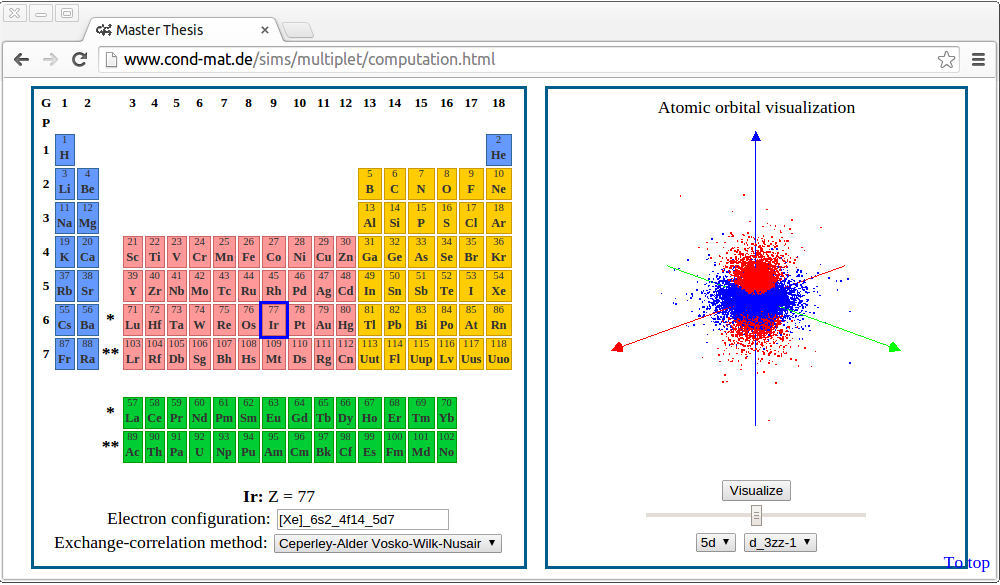
\includegraphics[width=0.8\textwidth]{js1}
  \[\texttt{www.cond-mat.de/sims/multiplet}\]
\end{frame}

\begin{frame}[t]
  \def\sqbox{
    \setlength{\unitlength}{1.5pt}
    \begin{picture}(10,10)
      \thicklines
      \color{red}
      \put(0,1){\line(1,0){12}}
      \put(12,1){\line(0,1){9}}
      \put(12,10){\line(-1,0){12}}
      \put(0,10){\line(0,-1){9}}
    \end{picture}
  }
  \frametitle{Comparison to NIST results}
  \footnotesize
  \centering
  \begin{tabular}{ c | c | r | r | r | r }
    \hline
    Elem & Orbital & My results & NIST results & Abs Error & Rel Error \\ \hline \hline
    H &  $1s^1$  &  $-0.233471$  &  $-0.233471$  &  0.000000  &  0.000000 \\  \hline
    C &  $1s^2$  &  $-9.947725$  &  $-9.947718$  &  0.000007  &  0.000001 \\ 
      &  $2s^2$  &  $-0.500866$  &  $-0.500866$  &  0.000000  &  0.000000 \\ 
      &  $2p^2$  &  $-0.199186$  &  $-0.199186$  &  0.000000  &  0.000000 \\ \hline
  Fe &  $1s^2$  &  $-254.225334$  &  $-254.225505$  &  0.000171  &  0.000001 \\ 
      &  $2s^2$  &  $-29.564863$  &  $-29.564860$  &  0.000003  &  0.000000 \\ 
      &  $2p^6$  &  $-25.551762$  &  $-25.551766$  &  0.000004  &  0.000000 \\ 
      &  $3s^2$  &  $-3.360622$  &  $-3.360621$  &  0.000001  &  0.000000 \\ 
      &  $3p^6$  &  $-2.187521$  &  $-2.187523$  &  0.000002  &  0.000001 \\
      &  $3d^6$  &  $-0.295047$  &  $-0.295049$  &  0.000002  &  0.000007 \\
      &  $4s^2$  &  $-0.197976$  &  $-0.197978$  &  0.000002  &  0.000010 \\
    \hline
  \end{tabular}
  
  \emph{\[\boxed{\text{Many-electron, mean-field!}}\]} \pause  
  
  \Put(37,258){\sqbox}
\end{frame}
